\section{Augenanalyse}
\label{ElSe}
Zur Bestimmung der Blickrichtung ist die Augenregion natürlich von besonderer Bedeutung. Aus diesem Grund werden die Landmarks der Augenregion nochmals gesondert betrachtet. Aufgrund der besonderen Bedeutung existiert eine große Anzahl an Algorithmen, die speziell auf eine hochgenaue Bestimmung von Augenmerkmalen optimiert sind, wie beispielsweise ElSe \cite{ElSe}, Goutam \cite{Eye_FastCorner}, Starburst \cite{Starburst} oder Swirski \cite{Swirski2012}.\\
Daher bestimmt OpenFace zusätzlich zu den 64 Landmarks, die das Gesicht beschreiben, weitere 28 Landmarks pro Auge, aus denen die Blickrichtung ermittelt wird. Um diese Augen-Landmarks zu bestimmen kommt ein weiteres CLNF zum Einsatz, das dafür trainiert wurde. Dabei zeigten die Vorabtests, dass die Detektion bei den getesteten kleinen Gesichtern unzureichend genau ausfällt.\\
Für die Bestimmung der Blickrichtung ist vor allem das Zentrum der Pupille bzw. Iris ausschlaggebend. Das Zentrum ergibt sich aus dem Umrissen (Landmarks) der Pupille bzw. Iris und muss möglichst exakt bestimmt sein, daher müssen diese aus dem Ergebnis von ElSe abgeleitet werden.\\
Um die Position der Landmarks zu verbessern, kann auf den Augenbereichen der ElSe-Algotithmus eingesetzt werden. Dieser Algorithmus basiert auf einem rechnerischen Ansatz und nicht auf Neuronen um die Umrisse der Pupille zu berechnen. Dieses Verfahren wurde gewählt, da es im Test \cite{ElSe} am besten abgeschnitten hat und direkt das Zentrum der Pupille liefert.
\subsection{Ellipse Selection for Robust Pupil Detection (ElSe)}
Bei realen Aufnahmen sind Bildfehler unvermeidlich, so können Reflektionen (Brille, Kontaktlinse usw.), Make-Up und körperliche Eigenschaften wie Augenfarbe die Detektion erschweren.\\
Der ursprüngliche ElSe-Algorithmus ist für Graubilder einer Eye-Tracking-Brille ausgelegt und optimiert, zudem ist es auf diesen Bildern zu einer Echtzeitauswertung in der Lage. Dieser Anwendungsbereich betrifft vor allem die hohe Qualität der Aufnahme im Bezug auf die Auflösung und die Infrarotbeleuchtung des Bildes. Die Infrarotbeleuchtung wird verwendet, damit das Auge ausreichend beleuchtet ist ohne den Probanden zu blenden.\\
Diese Voraussetzungen führen dazu, das die Detektionsleistung bei niedriger auflösenden Bildern rasch abnimmt. Da die Berechnung unabhängig der Landmarks ausgeführt wird, empfiehlt sich das Ergebnis zu überprüfen, damit die bestimmten Landmarks auch innerhalb der Augenhöhle liegen und grobe Fehler vermieden werden.\\
Für die Anwendung wurde der ursprüngliche ElSe-Algorithmus angepasst, um auf Farbbildern die nach Grau konvertiert wurden arbeiten zu können.\\
Als Ergebnis liefert ElSe eine Ellipse, die den Umriss der Pupille im Bild beschreibt. Aus dieser Ellipse können die Landmarks der Pupille abgeleitet werden.
Ein Problem das schon im Test aufgetreten ist, entsteht wenn der Farbunterschied zwischen Iris und Pupille recht gering ausfällt oder durch Reflektionen der Kantenverlauf gestört wird.\\
Für den Test im Paper wurden Bilder von $384\times 288$ Pixel Größe verwendet und im Vergleich zu den anderen Verfahren ist ElSe in den meisten Fällen überlegen, mit einer Verbesserung der Erkennungsrate um $14.53\%$ auf dem verwendeten Datensatz \cite{ElSe}.
\subsubsection{Pupille bestimmen mit Kantendetektion}
Da die Pupille als schwarzen Fleck im Bild dargestellt ist und die Iris einen helleren Farbton aufweist, wird ein Kantendetektor verwendet, der alle Pixel markiert, bei denen eine starke Farbänderung auftritt. Bei ElSe wird ein morphologischen Ansatz eingesetzt, von Relevanz sind nur zusammenhängende Kantenpixel um die Kante zwischen Pupille und Iris zu finden. Alle anderen Pixel können ignoriert werden, wobei jedes Kantenpixel als Startpunkt der Berechnung dienen kann.\\
Um jene Kantenpixel zu erhalten, die die Pupille beschreiben, wird versucht fortlaufende Kanten zu finden, die eine Ellipse bilden. Jene die nicht diesen Anforderungen entsprechen, können recht schnell ignoriert werden. Anschließend werden auch alle offenen Ellipsenverläufe und jene Kantenpixel die am meisten vom bestimmten Verlauf abweichen, verworfen.\\
Das beste Ergebnis aller bestimmten Ellipsen wird als Lösung verwendet.
\subsubsection{Grobe Bestimmung der Pupille}
\label{ElSe_Grob}
Sollte die Bestimmung der Ellipse, wie im letzten Kapitel beschreiben, scheitern, so wird das Zentrum des dunkelsten Kreises ermittelt. So ein Punkt kann immer gefunden werden, ist aber nicht zwingend die Pupille.\\
Auf einem verkleinerten Bild \autoref{img_else} (1) wird ein kreisförmiger Mean-Filter eingesetzt mit Ergebnis in \autoref{img_else} (3). Zur zweiten Faltung wird der Durchschnitt über ein Quadrat ohne inneren Kreis eingesetzt mit Ergebnis in \autoref{img_else} (2), wobei bei beiden Kreisen der selbe Radius verwendet wird.\\
Nun wird das Ergebnis des Quadratischen Mean-Filters invertiert \autoref{img_else} (4) und mittels Punkt-Multiplikation mit dem anderen Meanfilter zusammengebracht \autoref{img_else} (5). Im resultierendem Bild wird nun der höchste Wert gesucht, da dies das Zentrum des dunkelsten kreisförmigen Ortes im Bild ist.\\
Ergebnis des Beispiels ist als Kreuz in \autoref{img_else} (6) markiert. 
\begin{figure}
	\centering
	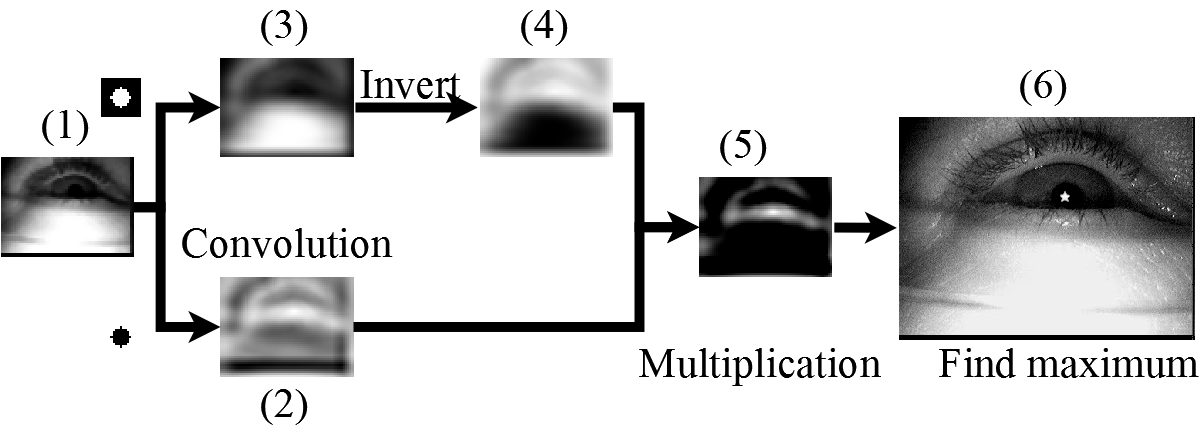
\includegraphics[width=0.8\linewidth]{img/ElSe}
	\caption{Ablauf der alternativen Berechnung zur Pupillen-Detektion von \cite{ElSe}}
	\label{img_else}
\end{figure}